\documentclass[7pt,letterpaper]{article}

\usepackage[pdftex]{graphicx}
\usepackage{float}
\usepackage{ulem}
\usepackage{listings}
\usepackage[in]{fullpage}
\usepackage{hyperref}
\usepackage{tipa}
\usepackage{natbib}
\usepackage[american]{babel} 
\usepackage{csquotes}
\usepackage{enumerate}
\usepackage{setspace}
\usepackage{qtree}

\pagestyle{empty}

\newcommand{\urlfootnote}[1]{\footnote{\url{#1}}}
\newcommand{\code}[1]{\texttt{#1}}
\newcommand{\authorInfo}[1]{\gdef\authInfo{#1}}
\newcounter{counter}

\title{KISS IDE}
\author{Braden McDorman}
\authorInfo{KISS Institute for Practical Robotics}

\begin{document}
	\makeatletter
	\noindent\begin{minipage}[l]{.8\textwidth}\begin{flushleft}\begin{small}
	\par\@author\vspace{.5em}
	
	\authInfo
	\end{small}\end{flushleft}\end{minipage}\vspace{.25in}
	
	\begin{center}
	\begin{Large}
	\textbf{\@title}
	\end{Large}
	\end{center}
	\makeatother
	
	\section{Overview}

	KISS IDE is an extensible IDE aimed at Robotics Development in C, C++, and Java. This document explains the internals of KISS, and should serve as
	a guide for anyone needing to modify its source.
	
	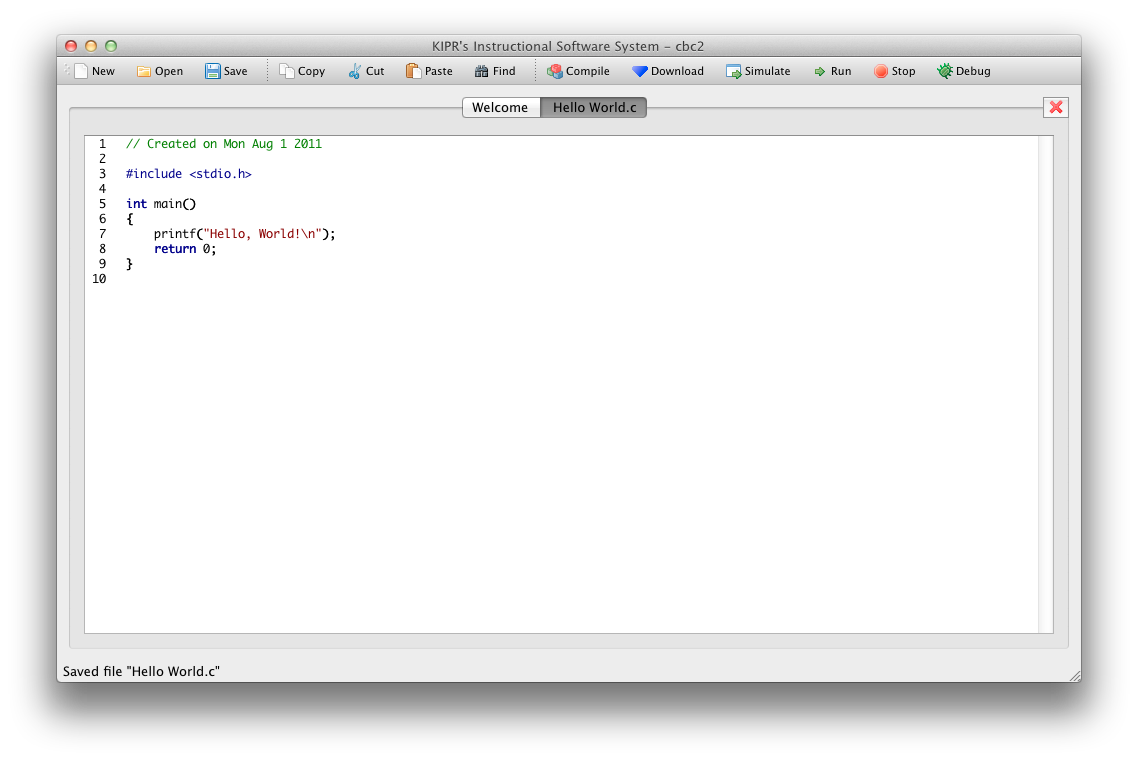
\includegraphics[width=1\textwidth]{KISS.png}

	\section{Tabs}
	
	A Tab is a class that may be managed and added to the \code{MainWindow} for viewing and interaction with the user. 
	For a class to identify itself as a Tab, it must implement the \code{Tab} interface.
	A Singleton is a global instance of a class, which can be retrieved using the \code{Singleton::ref()} static method.
	\textbf{\code{MainWindow} casts between \code{Tab} and \code{QWidget}, so a \code{Tab} needs to also implement \code{QWidget}.}
	These classes are implement \code{Tab} in KISS IDE:
	
	\subsection{Tab Classes}
	
	\setstretch{.5}
	\begin{description}
	\item[\code{SourceFile}] - The most important Tab. Allows editing of text, and interfacing with Targets.
	\item[\code{WebTab}] - Implements a simple Web Browser. Used for manuals and Botball Community.
	\item[\code{WelcomeTab}] - Extends \code{WebTab}, removing unnecessary functionality and loading the built-in Welcome HTML.
	\item[\code{VideoPlayerTab}] - Implements a Video Player on top of Phonon. To be used for lessons and other media.
	\item[\code{Repository}] - A graphical front-end to \code{KISSArchive}. Also allows downloading of packages from Repositories.
	\end{description}
	\singlespacing
	
	\subsection{Tab Usage}
	
	\lstset{language=C++,caption={The Tab Class},label=The Tab Class}
	\begin{lstlisting}
class Tab
{
public:	
	virtual void activate() = 0;
	virtual void addActionsFile(QMenu* file) = 0;
	virtual void addActionsEdit(QMenu* edit) = 0;
	virtual void addActionsHelp(QMenu* help) = 0;
	virtual void addOtherActions(QMenuBar* menuBar) = 0;
	virtual void addToolbarActions(QToolBar* toolbar) = 0;
	virtual bool beginSetup() = 0;
	virtual void completeSetup() = 0;
	virtual bool close() = 0;

	virtual void refreshSettings() = 0;
};
	\end{lstlisting}
	\vspace{.25in}
	
	\setstretch{.5}
	\begin{description}
	\item[\code{activate()}] - Called every time the tab becomes visible.
	\item[\code{addActionsFile(QMenu* file)}] - Passes \code{QMenu*} to add actions to the File menu.
	\item[\code{addActionsEdit(QMenu* edit)}] - Passes \code{QMenu*} to add actions to the Edit menu.
	\item[\code{addActionsHelp(QMenu* help)}] - Passes \code{QMenu*} to add actions to the Help menu.
	\item[\code{addOtherActions(QMenuBar* menuBar)}] - Allows other menus to be added to the menu bar.
	\item[\code{addToolbarActions(QToolBar* toolbar)}] - Allows actions to be placed in the tool bar.
	\item[\code{beginSetup()}] - A Tab should return \code{true} if setup was successful. \code{false} will prevent the Tab from opening.
	\item[\code{completeSetup()}] - Useful for setting Tab name. Tab has been added to the \code{MainWindow} at this point.
	\item[\code{close()}] - A Tab should return \code{true} if it may be closed. \code{false} otherwise. Prompt for save here.
	\item[\code{refreshSettings()}] - Should be a public slot in a Tab's implementation. Called when settings are updated.
	\end{description}
	\singlespacing
	
	\subsection{WebTab KISS URLs}
	
	WebTab allows HTML to modify the IDE's state through the use of special URLs. These URLs begin with \code{kiss://}.
	\code{kiss://command\#param}, where the scheme is \code{kiss}, \code{command} is the authority, and \code{param} is
	the URL's fragment.
	
	\setstretch{.5}
	\begin{description}
	\item[\code{kiss://new}] - Create new file with template.
	\item[\code{kiss://open}] - Shows open file dialog.
	\item[\code{kiss://settings}] - Show settings dialog.
	\item[\code{kiss://newbrowser\#http://google.com/}] - Creates a new browser, and loads google.com
	\item[\code{kiss://openfile\#path/to/file}] - Open file in new source tab.
	\item[\code{kiss://video\#path/to/video}] - Plays video in new video tab.
	\item[\code{kiss://external\#path/to/file}] - Opens a file in its default editor. (e.g. PDFs opened in Preview)
	\end{description}
	\singlespacing
	

	\section{Singletons}
	
	The Concept of a Singleton is an important one in KISS IDE. Several classes use Singletons as their base.
	A Singleton is a global instance of a class, which can be retrieved using the \code{Singleton::ref()} static method.
	These classes implement \code{Singleton} in KISS IDE:
	
	\subsection{Singleton Classes}
	
	\setstretch{.5}
	\begin{description}
	\item[\code{MainWindow}] - Manages Tabs and Opens Files.
	\item[\code{PluginManager}] - An interface for plugin loaders. This is implemented by \code{LexerManager} and \code{TargetManager}.
	\item[\code{LexerManager}] - Manages Loading of \code{LexerSpec} plugins.
	\item[\code{TargetManager}] - Manages loading of Target plugins.
	\item[\code{SourceFileShared}] - A Shared object used to store some common functionality for all \code{SourceFile} tabs.
	For example, Pixmaps and the Debugger are shared resources among all \code{SourceFile} instances.
	\end{description}
	\singlespacing
	
	Singletons for Plugins are necessary, as plugins are inherently single instances. Thus, plugins each have one instance for the entire execution of KISS.
	

	\section{Plugins}
	
	\code{PluginManager} is the interface used by both \code{TargetManager} and \code{LexerManager} to load plugins.
	An implementing class must implement \code{getExpectedLocation(const QString\& name)}, which returns the directory to look
	for a plugin with the given \code{name}. In \code{TargetManager}, this returns \code{targets/\$\{name\}}, while in \code{LexerManager} this returns
	\code{lexers}. PluginManager also relies on the implementer to \code{unloadAll()} plugins on destruction.
	
	\subsubsection{Plugin Naming}
	\code{PluginManager} expects plugins to follow the naming scheme \code{lib\$\{name\}\_plugin.\$\{os\_lib\_ext\}}. This is the default on Mac OS X and Unix, but Windows
	requires some modification. Here is an example of how this is achieved in the python target:
	
	\lstset{caption={Python Target},label=Python Target}
	\begin{lstlisting}
TARGET = $$qtLibraryTarget(python_plugin)
win32:TARGET = $$qtLibraryTarget(libpython_plugin)
	\end{lstlisting}
	\vspace{.25in}
	
	\subsection{Lexers}
	The Lexer system has several parts, including \code{Lexer}, \code{LexerProvider}, \code{LexerSpec}, and \code{LexerManager}. This may be quite confusing at first glance,
	but provides a robust way to interface with QScintilla. \code{Lexer} implements \code{QsciLexer} for wrapping \code{LexerSpec} classes. 
	\code{LexerSpec} is a struct that a plugin developer should implement to highlight syntax. \code{LexerProvider} is the interface for plugins, which
	gives you a \code{LexerSpec} to configure in the \code{init()} method of the plugin. \code{LexerManager} manages the loading of \code{LexerProvider}s.
	
	\subsection{LexerManager Notes}
	\code{LexerManager} keeps track of lexer extensions in a thin layer on top of \code{PluginManager}. This is necessary because lexers can be registered to
	multiple extensions, while \code{PluginManager} expects a 1:1 mapping. It is recommended you use the \code{lexerSpec(const QString\& ext)} function to return the
	appropriate LexerProvider for a given extension rather than \code{get(const QString\& name)}.

	\section{KISS Archives}
	KISS Archives are a way to install and uninstall optional components into KISS. All targets, lexers, and video lessons build KISS Archives, some of which are
	preinstalled for distribution. The \code{KissArchive} class provides several static methods for the manipulation and creation of these archives. KISS also has a
	basic CLI for these commands. The currently installed packages are kept track of in an \code{installed} file located in the working directory of KISS.
	Just to be safe, installing/uninstalling KISS Archives unloads all plugins. The easiest way to reload KISS at this point is a restart of KISS.
	
	\lstset{language=C++,caption={KISS Archive Header},label=KISS Archive Header}
	\begin{lstlisting}
struct KissReturn 
{
	bool error;
	QString message;
};

class KissArchive 
{
public:
	static KissReturn create(const QString& name, unsigned version, 
		const QStringList& platforms, const QStringList& files, 
		QIODevice* out);
	static KissReturn install(QIODevice* in);
	static KissReturn uninstall(const QString& name);
	static QStringList list(QIODevice* in);
	static const unsigned version(const QString& name);
	static QStringList installed();
};
	\end{lstlisting}
	\vspace{.25in}
	
	\subsection{CLI Interface}
	
	\setstretch{.5}
	\begin{description}
	\item[\code{KISS --createArchive name version platforms contents output.kiss}] - Creates a KISS Archive
	\item[\code{KISS --uninstall name}] - Uninstalls a kiss archive in the working directory.
	\item[\code{KISS --install file.kiss}] - Installs a kiss archive in the working directory.
	\item[\code{KISS --list}] - Lists installed KISS Archives
	\end{description}
	\singlespacing
	
	\subsubsection{Example Creating KISS Archive}
	In this example, we create a \code{contents} file containing newline delimited files to add to a KISS Archive.
	
	\lstset{language=bash,caption={Building KISS Archive for Windows},label=Building KISS Archive for Windows}
	\begin{lstlisting}
find * -type f > contents
${KISS}/deploy/KISS --createArchive name 1 win contents test_archive_win.kiss
	\end{lstlisting}
	\vspace{.25in}
	In this example, we use \code{win,osx,nix} rather than \code{win} to specify we want all platforms to be supported.
	
	\lstset{language=bash,caption={Building KISS Archive for All Platforms},label=Building KISS Archive for All Platforms}
	\begin{lstlisting}
find * -type f > contents
${KISS}/deploy/KISS --createArchive name 1 win,osx,nix contents test_archive.kiss
	\end{lstlisting}
	\vspace{.25in}
	\textbf{On Mac OS X, the path of KISS is \$\{KISS\}/deploy/KISS.app/Contents/MacOS/KISS}
	
	\subsection{Repositories}
	A repository simply is a remote directory served over HTTP. This directory is required to have an \code{available.lst} file in it, which specifies the packages
	available for download. The format of the \code{available.lst} file is as follows: \code{os<tab>name<tab>version<tab>file}
	
	\subsubsection{Example available.lst}
	\lstset{caption={Example available.lst},label=Example available.lst}
	\begin{lstlisting}
win	cbc2	1	cbc2_target_win.kiss
osx	cbc2	1	cbc2_target_osx.kiss
nix	cbc2	1	cbc2_target_nix.kiss
win	c lexer	1	c_lexer_win.kiss
	\end{lstlisting}
	\vspace{.25in}
	

	\section{Targets}
	Targets implement the \code{TargetInterface}, which allows the target to specify the actions it can perform, and perform them.
	The TargetInterface passes a port name with most functions, as Targets are not bound to any specific file or port.
	The \code{Target} class stores a port, and provides wrappers for all TargetInterface functions. It is recommended code wishing to
	use a Target use the \code{Target} class instead of a \code{TargetInterface} directly.
	
	\lstset{language=C++,caption={Target Class},label=Target Class}
	\begin{lstlisting}
class Target : public QObject
{
public:
	Target(QObject *parent = 0);

	bool setTargetFile(const QString& filename);
	QMap<QString, QString> targetManualPaths();
	QString requestFilePath();

	QStringList 	errorMessages();
	QStringList 	warningMessages();
	QStringList 	linkerMessages();
	QStringList 	verboseMessages();
	QList<QAction*> actionList();

	QStringList sourceExtensions();
	QString defaultExtension();
	bool cStyleBlocks();
	
	bool hasDownload();
	bool hasCompile();
	bool hasRun();
	bool hasStop();
	bool hasSimulate();
	bool hasDebug();
	bool hasUi();

	bool compile(const QString& filename);
	bool download(const QString& filename);
	bool run(const QString& filename);
	void stop();
	bool simulate(const QString& filename);
	DebuggerInterface* debug(const QString& filename);
	Tab* ui();

	bool hasRequestFile();
	QStringList requestDir(const QString&);
	QByteArray requestFile(const QString&);

	bool error();

	bool hasPort();
	void setPort(const QString& port);
	const QString& port() const;
};
	\end{lstlisting}
	\vspace{.25in}
	
	\subsection{Layout of a Target}
	\setstretch{.5}
	\begin{description}
	\item[\code{kiss-targets/name}] - Target directory
	\item[\code{kiss-targets/name/name.pro}] - Qt project file for building
	\item[\code{kiss-targets/name/name.target}] - Loaded by KISS at runtime for target information
	\item[\code{kiss-targets/name/name.api}] - Used for auto-completion in the editor.
	\item[\code{kiss-targets/name/src/*}] - Source Files.
	\item[\code{kiss-targets/name/templates/*}] - Templates for New File dialog
	\end{description}
	\singlespacing
	
	\subsubsection{Compiled Target Layout}
	\setstretch{.5}
	\begin{description}
	\item[\code{targets/name}] - Target directory (\code{kiss-targets/root/targets})
	\item[\code{targets/name/libname\_plugin.dylib}] - Plugin shared library (dylib on Mac OS X)
	\item[\code{targets/name/name.target}]
	\item[\code{targets/name/name.api}]
	\item[\code{kiss-targets/name/templates/*}] - Templates for New File dialog
	\end{description}
	\singlespacing
	
	\subsection{Target File}
	
	\lstset{caption={Example Target File},label=Example Target File}
	\begin{lstlisting}
[General]
description=A Description of the Target
display_name=CBCv2
extensions=C Sources (*.c *.h)|C++ Sources (*.cpp *.h *.hpp)
name=cbc2
port_dialog=true
default_extension=c
c_style_blocks=true
request_file_path=/mnt/browser/stage

[Manuals]
Manual=targets/cbc2/manual/cbcmanual.html
Sensors and Motors Manual=targets/cbc2/manual/Sensor_and_Motor_Manual_BB2011.pdf
Video Lessons=videos/videos.html

[win]
cflags=-Wimplicit -include stdio.h ...
include_dirs=targets/gcc/include targets/cbc2/include
lflags=-lcbc2_sim -lkiss -lglfw -lGLee -lopengl32 ...
lib_dirs=targets/gcc/lib targets/cbc2/lib

[osx]
cflags=-arch i386 -Wimplicit -include stdio.h ...
include_dirs=targets/gcc/include targets/cbc2/include
lflags=-arch i386 -lcbc2_sim -lGLee -lkiss ...
lib_dirs=targets/gcc/lib targets/cbc2/lib

[nix]
cflags=-Wimplicit -include stdio.h ...
include_dirs=targets/gcc/include targets/cbc2/include
lflags=-lcbc2_sim -lkiss ...
lib_dirs=targets/gcc/lib targets/cbc2/lib
	\end{lstlisting}
	\vspace{.25in}
	
	\subsubsection{Target File Options}
	\setstretch{.5}
	\begin{description}
	\item[\code{General/description}] - Description to appear on hover in \code{TemplateDialog}.
	\item[\code{General/display\_name}] - Name to appear in \code{TemplateDialog}.
	\item[\code{General/extensions}] - Pipe delimited source files this target is allowed to open.
	\item[\code{General/name}] - Name.
	\item[\code{General/port\_dialog}] - True if needs port dialog (for downloading, running, etc.)
	\item[\code{General/default\_extension}] - Default lexerspec to use, unless the template specifies otherwise.
	\item[\code{General/c\_style\_blocks}] - If the language uses curly brackets in code. Used to turn on/off ``Indent All".
	\item[\code{General/request\_file\_path}] - The remote path to look for files by default.
	\item[\code{Manuals}] - Holds list of manuals, in the format \code{Name=Path/to/Manual}. Will not show non-existent manual.
	\end{description}
	\singlespacing
	The other sections are left to the target to process, such as compiler and linker flags.
	
	\subsection{CBCv2}
	The CBCv2 target is very similar to GCC, and requires GCC to be installed to work.
	The CBCv2 target uses cbcserial to communicate with the CBC.
	
	\section{Templates}
	Templates are the files that appear in the \code{TemplateDialog} when creating a new file. A template has the extension \code{.template}
	and has the same name that will be displayed in the \code{TemplateDialog}. For example, \code{Hello World.template} will appear in the 
	\code{TemplateDialog} as ``Hello World". Templates also have \code{.png} icon by the same name in the same directory. If this icon is not
	found, \code{TemplateDialog} falls back on a \code{Default.png} in the same directory. If \code{Default.png} doesn't exist, no icon is 
	displayed. Templates may be located in the \code{target/templates} directory, or one subdirectory lower. For example, 
	\code{target/templates/Examples/Turn Left.template} is also valid, and will appear in an ``Examples" folder in the \code{TemplateDialog}.
	
	\vspace{.25in}
	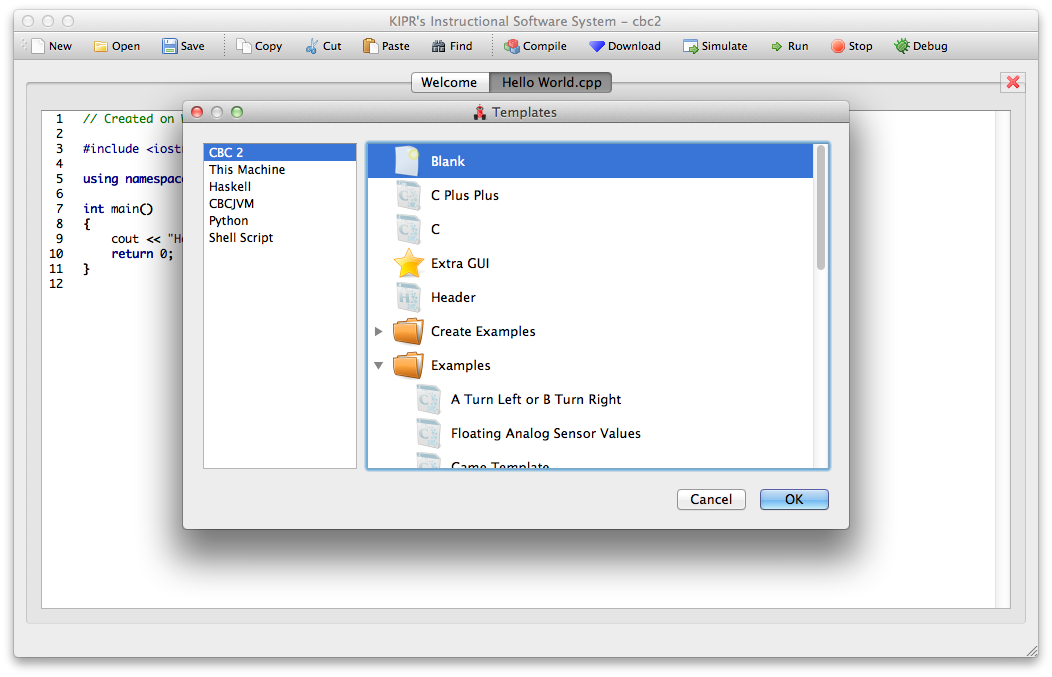
\includegraphics[width=1\textwidth]{KISSTemplates.png}
	
	\subsection{Template Metadata}
	Template files usually contain exactly the text you want loaded into the editor, but KISS allows us to specify some information in a template file.
	
	\setstretch{.5}
	\begin{description}
	\item[\code{KISS\_LEXER <lexer\_name>}] - Specifies the lexerspec to use instead of the target's default.
	\item[\code{KISS\_END\_META}] - Ends the meta section of a template file, which is always the top of the file.
	If no metadata is necessary, this keyword may be omitted.
	\item[\code{KISS\_DATE}] - Inserts the date at any place in the file.
	\end{description}
	\singlespacing
	
	\lstset{caption={Example Template with Metadata},label=Example Template with Metadata}
	\begin{lstlisting}
KISS_LEXER cpp
END_KISS_META
// Created on KISS_DATE

#include <iostream>

using namespace std;

int main() 
{
	cout << "Hello, World!" << endl;
	return 0;
}
	\end{lstlisting}
	\vspace{.25in}
	
	\lstset{caption={Example Template without Metadata},label=Example Template without Metadata}
	\begin{lstlisting}
// Created on KISS_DATE

#include <stdio.h>

int main() 
{
	printf("Hello, World!\n");
	return 0;
}
	\end{lstlisting}
	\vspace{.25in}
	
	\section{Serial Communication with the CBC}
	Serial Communication has been largely rewritten in KISS IDE.
	You may link to the \code{cbcserial} library in \code{kiss-targets/libraries} to use serial communication.
	\code{SerialClient} exposes a few useful functions for serial interaction:
	
	\setstretch{.5}
	\begin{description}
	\item[\code{setPort(const QString\& port)}] - Set port to communicate over.
	\item[\code{sendCommand(quint16 command, const QByteArray\& data = "")}] - 
	Sends a command (which is a unique unsigned short) and an associated byte array.
	\item[\code{waitForResult(quint16 command, QByteArray\& data)}] - 
	Waits for a command with the specified unsigned short to be sent from the CBC. 
	Data is set to the CBC's response
	\item[\code{sendFile(const QString\& name, const QString\& destination)}] - Just a wrapper for \code{KISS\_SEND\_FILE\_COMMAND}. 
	Name is the path to a file, while destination is the local CBC path to write to.
	\end{description}
	\singlespacing
	
	\subsection{Commands}
	\vspace{.25in}
	\setstretch{.5}
	\begin{description}
	\item[\code{KISS\_SEND\_FILE\_COMMAND 	1}] - Sends file to CBC
	\item[\code{KISS\_REQUEST\_FILE\_COMMAND 	2}] - Request file response from CBC
	\item[\code{KISS\_LS\_COMMAND 		3}] - Request ls of given directory
	\item[\code{KISS\_RUN\_COMMAND 		4}] - Run given file
	\item[\code{KISS\_STOP\_COMMAND 		5}] - Stop currently running program
	\item[\code{KISS\_EXECUTE\_COMMAND 		6}] - Execute arbitrary shell command
	\item[\code{KISS\_COMPILE\_COMMAND 		7}] - Compile given file
	\item[\code{KISS\_CREATE\_PROJECT\_COMMAND 	8}] - Create given project name
	\item[\code{KISS\_PRESS\_A\_COMMAND 		9}] - Simulate A press
	\item[\code{KISS\_PRESS\_B\_COMMAND 		10}] - Simulate B press
	\item[\code{KISS\_PRESS\_LEFT\_COMMAND 	11}] - Simulate Left press
	\item[\code{KISS\_PRESS\_RIGHT\_COMMAND 	12}] - Simulate Right press
	\item[\code{KISS\_PRESS\_UP\_COMMAND 		13}] - Simulate Up press
	\item[\code{KISS\_PRESS\_DOWN\_COMMAND 	14}] - Simulate Down press
	\item[\code{KISS\_RELEASE\_A\_COMMAND 		15}] - Simulate A release
	\item[\code{KISS\_RELEASE\_B\_COMMAND 		16}] - Simulate B release
	\item[\code{KISS\_RELEASE\_LEFT\_COMMAND 	17}] - Simulate Left release
	\item[\code{KISS\_RELEASE\_RIGHT\_COMMAND 	18}] - Simulate Right release
	\item[\code{KISS\_RELEASE\_UP\_COMMAND 	19}] - Simulate Up release
	\item[\code{KISS\_RELEASE\_DOWN\_COMMAND 	20}] - Simulate Down release
	\item[\code{KISS\_GET\_STATE\_COMMAND 		21}] - Request State information (sensors and motor values)
	\item[\code{KISS\_GET\_STDOUT\_COMMAND 	22}] - Get stdout change since last request
	\item[\code{KISS\_DELETE\_FILE\_COMMAND 	23}] - Delete file at given file path
	\item[\code{KISS\_MKDIR\_COMMAND 		24}] - Make given directory

	\item[\code{CBC\_REQUEST\_FILE\_RESULT 	127}] - Response to Request File
	\item[\code{CBC\_LS\_RESULT 			128}] - Response to ls
	\item[\code{CBC\_EXECUTE\_RESULT 		129}] - Response to arbitrary command
	\item[\code{CBC\_COMPILE\_SUCCESS\_RESULT 	130}] - Response to compile
	\item[\code{CBC\_STATE\_RESULT 		131}] - Response to state request
	\item[\code{CBC\_STDOUT\_RESULT 		132}] - Response to stdout request
	\end{description}
	\singlespacing
	
	\subsection{Useful References for Serial Communication}
	\setstretch{.5}
	\begin{description}
	\item[\code{kiss-targets/libraries/cbcserial/SerialClient.cpp}] - Communicates with the CBCv2
	\item[\code{kiss-targets/libraries/cbcserial/QSerialPort.cpp}] - Makes serial communication cross-platform
	\item[\code{cbc/cbcui/src/Serial/SerialServer.cpp}] - The CBC side of serial communication. Shows how each command's data should be packed.
	\end{description}
	\singlespacing
	

	\section{Building KISS}
	
	\subsection{Mac OS X}
	\begin{list}{Step \arabic{counter}:~}{\usecounter{counter}}{}
	\item Download and Install the Cocoa Version (Carbon for PPC) of Qt from \newline
	\url{http://qt.nokia.com/downloads/qt-for-open-source-cpp-development-on-mac-os-x}
	\item Download and Extract QScintilla from \newline
	\url{http://www.riverbankcomputing.co.uk/software/qscintilla/download}
	\item \code{cd \$\{qscintilla\}/Qt4}
	\item \code{nano qscintilla.pro} \newline
	Change \code{dll} to \code{staticlib} under \code{CONFIG}. \newline
	Remove \code{QSCINTILLA\_MAKE\_DLL} from \code{DEFINES}. \newline
	\code{Ctrl-X, Y, Enter} to Save and Exit.
	\item \code{qmake -spec macx-g++}
	\item \code{make}
	\item \code{sudo make install}
	\item \code{cd \$\{development\}}
	\item \code{git clone git@github.com:kissInstitute/kiss.git}
	\item \code{git clone git@github.com:kissInstitute/kiss-targets.git}
	\item \code{git clone git@github.com:kissInstitute/kiss-lexers.git}
	\item \code{echo "KISS=\$\{development\}/kiss" > kiss-lexers/kiss.pri} (Absolute path to kiss)
	\item \code{echo "KISS=\$\{development\}/kiss" > kiss-targets/kiss.pri} (Absolute path to kiss)
	\item \code{cd kiss}
	\item \code{sh scripts/buildAll.sh ../kiss-targets ../kiss-lexers} (Deploys kiss to \code{kiss/deploy})
	\item Open deploy/KISS.app and install the packages you want to deploy with.
	\item \code{sh scripts/osx\_packager.sh version\_number}
	\item Your KISS dmg is now ready in the releases folder.
	\end{list}
	
	\subsection{Windows}
	\textbf{The Windows build piggy-backs off of the unix msysgit environment, so all commands should be executed from a msysgit prompt.}
	\begin{list}{Step \arabic{counter}:~}{\usecounter{counter}}{}
	\item Download and Install msysgit from \newline
	\url{http://code.google.com/p/msysgit/downloads/list}
	\item Download and Install GNU Make from (\textbf{Install to C:\textbackslash gnuwin32}) \newline
	\url{http://gnuwin32.sourceforge.net/packages/make.htm} 
	\item Download and Install Qt from (\textbf{Install to C:\textbackslash Qt}) \newline
	\url{http://qt.nokia.com/downloads/sdk-windows-cpp}
	\item Download and Extract QScintilla from \newline
	\url{http://www.riverbankcomputing.co.uk/software/qscintilla/download} to \code{C:\textbackslash Projects\textbackslash}
	\item Download and Install NSIS from \newline
	\url{http://nsis.sourceforge.net/Download}
	\item Right Click on Computer, Properties, Advanced System Settings, Environment Variables, Path, Edit... (On Windows Vista or 7)
	\item Append \code{;C:\textbackslash Qt\textbackslash mingw\textbackslash bin;C:\textbackslash Qt\textbackslash Desktop\textbackslash Qt\textbackslash \$\{version\}\textbackslash mingw\textbackslash bin;C:\textbackslash gnuwin32\textbackslash bin}
	\item \code{mkdir -p /c/Projects}
	\item \code{cd /c/Projects}
	\item \code{cd QScintilla*/Qt4}
	\item \code{qmake}
	\item \code{make}
	\item \code{cp -R Qsci /c/Qt/mingw/include}
	\item \code{cp releases/qscintilla2.dll /c/Qt/mingw/bin}
	\item \code{cd /c/Projects}
	\item \code{git clone git@github.com:kissInstitute/kiss.git}
	\item \code{git clone git@github.com:kissInstitute/kiss-targets.git}
	\item \code{git clone git@github.com:kissInstitute/kiss-lexers.git}
	\item \code{echo "KISS=../../kiss" > kiss-lexers/kiss.pri}
	\item \code{echo "KISS=../../kiss" > kiss-targets/kiss.pri}
	\item \code{mkdir -p kiss-targets/root/targets}
	\item Copy distribution mingw to kiss-targets/gcc
	\item \code{cd kiss}
	\item \code{mkdir depends}
	\item \code{mkdir releases}
	\item You will need to populate \code{depends} with \code{libgcc\_s\_dw2-1.dll}, \code{mingwm10.dll},
		\code{phonon\_ds94.dll}, \code{phonon4.dll}, \code{qscintilla2.dll}, \code{QtCore4.dll}, \code{QtGui4.dll},
		\code{QtNetwork4.dll}, \code{QtWebKit4.dll}
	\item \code{sh scripts/buildAll.sh ../kiss-targets ../kiss-lexers} (Deploys kiss to \code{kiss/deploy})
	\item Right click on kiss/scripts/KISS.nsi, Compile NSIS Script (Choose Compressor)
	\item Choose LZMA (Solid) as compressor.
	\item Your KISS installer is now built in the releases folder.
	\end{list}
	
	\subsection{Linux}
	\begin{list}{Step \arabic{counter}:~}{\usecounter{counter}}{}
	\item Install Qt4 and libqscintilla2 development packages using system package manager
	\item \code{cd \$\{development\}}
	\item \code{git clone git@github.com:kissInstitute/kiss.git}
	\item \code{git clone git@github.com:kissInstitute/kiss-targets.git}
	\item \code{git clone git@github.com:kissInstitute/kiss-lexers.git}
	\item \code{echo "KISS=\$\{development\}/kiss" > kiss-lexers/kiss.pri} (Absolute path to kiss)
	\item \code{echo "KISS=\$\{development\}/kiss" > kiss-targets/kiss.pri} (Absolute path to kiss)
	\item \code{cd kiss}
	\item \code{sh scripts/buildAll.sh ../kiss-targets ../kiss-lexers} (Deploys kiss to \code{kiss/deploy})
	\item Open deploy/KISS and install the packages you want to deploy with.
	\end{list}
	
\end{document}